\chapter{Theoretische Grundlagen}

\section{Canny-Kantendetektion}

Der Canny-Kantendetektor, erstmals von John Canny im Jahr 1986 vorgestellt \cite{canny_computational_1986}, stellt einen mehrstufigen Algorithmus dar, dessen Grundlage eine formale mathematische Definition der Zielsetzung eines idealen Kantendetektors bildet. Canny formulierte die Kantenerkennung als Optimierungsproblem und leitete drei mathematische Kriterien ab, denen ein optimaler Detektor für stufenförmige Kanten genügen muss. Aus diesen Kriterien wurde eine spezifische Operatorform hergeleitet, sodass der Algorithmus als deren direkte technische Umsetzung zu verstehen ist.

\begin{enumerate}
  \item \textbf{Gute Erkennungrate:}  Die Fehlerwahrscheinlichkeit, echte Kanten zu übersehen oder fälschlicherweise Nicht-Kanten zu markieren, muss minimiert werden.
  \item \textbf{Gute Lokalisierung:} Die markierte Kantenposition soll eine minimale Abweichung vom tatsächlichen Kantenzentrum aufweisen.
  \item \textbf{Eindeuige Antwort:} Der Detektor darf auf eine einzelne Kante nicht mit mehreren lokalen Maxima antworten.
\end{enumerate}

Der Canny-Kantendetektor arbeitet in vier aufeinanderfolgenden Schritten. Zunächst wird das Eingabebild durch Faltung mit einem Gauß-Filter geglättet, um hochfrequentes Rauschen zu unterdrücken, wobei die Standardabweichung $\sigma$ als zentraler Parameter die Robustheit gegenüber der Lokalisierungsgenauigkeit abwägt. Anschließend werden für jeden Pixel Kantenstärke und Kantenrichtung aus dem Gradienten des geglätteten Bildes berechnet, bevor im dritten Schritt die Nicht-Maxima-Unterdrückung die Kantenantworten durch Beibehaltung ausschließlich lokaler Maxima entlang der
Gradientenrichtung auf eine Pixelbreite reduziert.

Den abschließenden und für die Qualität des Ergebnisses entscheidenden Schritt bildet die Klassifikation mittels Hysterese-Schwellwertverfahren. Dieses verwendet zwei Schwellwerte $T_1$ und $T_2$, wobei Pixel oberhalb von $T_1$ als sichere Kanten klassifiziert werden, während Pixel im Intervall $[T_2,\, T_1]$ nur dann akzeptiert werden, wenn sie räumlich mit einer sicheren Kante verbunden sind. Durch diesen zweistufigen Mechanismus wird das als \textit{Streaking} bekannte Abreißen von Kantenzügen infolge lokaler Schwankungen der Kantenstärke zuverlässig verhindert.

\section{Hough Transformation}

In diesem Kapitel werden die Grundlagen der \ac{HT} vermittelt. Dabei wird zuerst die Funktionsweise der Erkennung von Linien und anschließend die Erkennung von Kreisen erklärt.

\label{Hough-chapter}

\subsection{Erkennung von Linien}

Die \ac{HT} ist ein grundlegendes Verfahren der digitalen Bildverarbeitung und des maschinellen Sehens, das der Erkennung geometrischer Formen und Muster in Bilddaten dient. Sie wurde ursprünglich von Paul Hough im Jahr 1962 in einem Patent zur Erkennung komplexer Muster in Blasenkammeraufnahmen vorgestellt. \cite{illingworth_survey_1988,hough_method_1962}.

Die Funktionsweise der \ac{HT} veranschaulicht die Abbildung \ref{Hough Prinzip}. Dabei werden Punkte aus dem ursprünglichen Bildraum in den Parameterraum transformiert. Der Bildraum ist im klassischen Sinne der Raum in dem Punkte in x und y Koordinaten angegeben werden. Der Parameterraum bezieht sich hingegen auf die beiden Parameter m und c einer Geraden. Eine wichtige Eigenschaft hierbei ist, dass Punkte im Bildraum durch die Transformation zu Geraden im Parameterraum werden. Der Schnittpunkt der Geraden im Parameterraum gibt die Parameter m und c der Geraden an, durch die die jeweiligen Punte im Bildraum verbunden werden. \cite{illingworth_survey_1988}

Um die \ac{HT} berechnen zu können, wird der Parameterraum als ein mehrdimensionales Array, das sogenannte Akkumulator-Array, dargestellt, wobei jedes Element hochgezählt wird, sobald eine Gerade dadurch verläuft. Die Erkennung von Hochpunkten ist im Parameterraum einfacher und rechnerisch weniger fordernd als im Bildraum. \cite{illingworth_survey_1988} Die Tabelle \ref{Accumulator-Array} dient dafür als Veranschaulichung.


\begin{figure}[H]
\centering
\begin{subfigure}{0.4\textwidth}
\centering
\begin{tikzpicture}
  \draw[->] (-3,0) -- (3,0) node[right] {$x$};
  \draw[->] (0,-3) -- (0,3) node[above] {$y$};

  \draw[dashed] (-2,-2) -- (3,3);

  \fill (1,1) circle (2pt) node[right] {$P_1(1, 1)$};
  \fill (2,2) circle (2pt) node[right] {$P_2(2, 2)$};

  \fill (-2,1) circle (2pt) node[above right] {$P_3(-2, 1)$};
  
\end{tikzpicture}
\caption{Punkte im Bildraum}
\label{a}
\end{subfigure}
\begin{subfigure}{0.4\textwidth}
\centering
\begin{tikzpicture}

% Achsen
\draw[->] (-3,0) -- (3,0) node[right] {$m$};
\draw[->] (0,-3) -- (0,3) node[above] {$c$};

% Gerade f(x) = -x + 1
\draw[domain=-2:3] plot (\x, {-\x + 1})
      node[right] {$f(x)=-x+1$};

% Gerade g(x) = -x + 2
\draw[domain=-1:3] plot (\x, {-\x + 2})
      node[right] {$g(x)=-x+2$};

% Gerade h(x) = 2x + 1
\draw[domain=-2:1] plot (\x, {2*\x + 1})
      node[right] {$h(x)=2x+1$};

\fill (0,1) circle (2pt);

\end{tikzpicture}
\caption{Punkte im Parameterraum}
\label{b}
\end{subfigure}
\caption{Grundprinzip der Hough-Transformation}
\label{Hough Prinzip}
\end{figure}

\begin{table}[H]
\centering
\renewcommand{\arraystretch}{1.3}
\setlength{\tabcolsep}{8pt}

\begin{tabular}{cccccc}

1 & 0 & 1 & 0 & 0 & 0 \\
0 & 1 & 0 & 1 & 0 & 1 \\
0 & 0 & 1 & 0 & 2 & 0 \\
0 & 0 & 0 & 2 & 0 & 1 \\
0 & 0 & 1 & 0 & 1 & 0 \\
0 & 1 & 0 & 0 & 0 & 1 \\
1 & 0 & 0 & 0 & 0 & 0 \\
\end{tabular}

\caption{Accumulator-Array im Parameterraum $(m,c)$}
\label{Accumulator-Array}
\end{table}

In einer Veröffentlichung von Duda und Hart \cite{duda_use_1972} wurde vorgeschlagen, dass man statt der ursprünglichen Geradenform mit m und c die Normalform welche durch folgende Gleichung beschrieben wird nutzt. Dabei gibt $\rho$ den Abstand der Geraden zum Ursprung und $\theta$ den Winkel der Normalen zur Gerade im Intervall [0, $\pi$] an.

\[
\rho = x * cos(\theta) + y * sin(\theta)
\]

Dadurch wird ein Speicheraufwand von $n^2$ bei n Punkten vermieden, der bei der klassichen Methode durch Testen aller Punktpaare entsteht. Für diese Arbeit ist die Darstellung der Koordinaten in Normalform wichtig, da sie im Python Modul OpenCV ebenfalls zum Einsatz kommt. \cite{noauthor_opencv_nodate}

Für jeden Punkt ($x_0, y_0$) kann denmnach eine Menge von Geraden durch folgende Gleichung gefunden werden. Der Schnittpunkt mehrerer Koordinaten gibt die Gerade an, welche durch die jeweiligen Punkte verläuft. Die Abbildung \ref{Polarkoordinaten} veranschaulicht das Konzept.

\[
\rho = x_0 * cos(\theta) + _0 * sin(\theta)
\]

\begin{figure}[H]
\centering
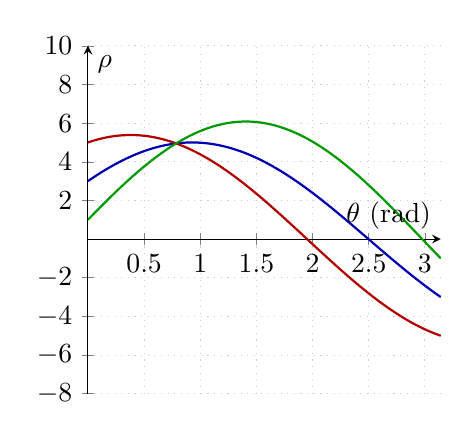
\begin{tikzpicture}
  \begin{axis}[
    width=0.5\textwidth,
    height=6cm,
    xmin=0, xmax=pi,
    ymin=-8, ymax=10,
    xlabel={$\theta$ (rad)},
    ylabel={$\rho$},
    xtick={0, 0.5, 1.0, 1.5, 2.0, 2.5, 3.0},
    ytick={-8,-6,-4,-2,0,2,4,6,8,10},
    axis lines=center,
    grid=major,
    grid style={dotted, gray!40},
    every axis plot/.style={thick},
  ]
    % Punkt (3,4): rho = 3cos(theta) + 4sin(theta)
    \addplot[domain=0:pi, samples=300, blue!70!black]
      {3*cos(deg(x)) + 4*sin(deg(x))};

    % Punkt (5,2): rho = 5cos(theta) + 2sin(theta)
    \addplot[domain=0:pi, samples=300, red!70!black]
      {5*cos(deg(x)) + 2*sin(deg(x))};

    % Punkt (1,6): rho = 1cos(theta) + 6sin(theta)
    \addplot[domain=0:pi, samples=300, green!60!black]
      {cos(deg(x)) + 6*sin(deg(x))};

  \end{axis}
\end{tikzpicture}
\caption{Parameterraum in Polarkoordinaten}
\label{Polarkoordinaten}
\end{figure}

\subsection{Erkennung von Kreisen}

Die Erkennung von Kreisen basiert auf demselben Prinzip wie die zuvor beschriebene Linienerkennung, jedoch wird anstelle der Geradengleichung die Kreisgleichung 
\[
(x_i - a)^2 + (y_i - b)^2 = r^2
\]

als parametrische Darstellung verwendet, wobei $a$ und $b$ die Koordinaten des Kreismittelpunkts und $r$ den Radius bezeichnen. $x_i$ und $y_i$ sind die Koordinaten eines auf dem Kreis liegenden Punktes $P_i$. Zur Reduktion der Problemkomplexität wird der Radius $r$ zunächst als bekannt vorausgesetzt, sodass der zweidimensionale Parameterraum ausschließlich durch die Mittelpunktkoordinaten $a$ und $b$ aufgespannt wird. Wie in Abbildung~\ref{fig:hough-transformation} dargestellt, wird jeder Bildpunkt im Parameterraum als Kreis repräsentiert, dessen Schnittpunkt mit den übrigen transformierten Punkten den gesuchten Kreismittelpunkt bestimmt. \cite{illingworth_survey_1988}

\begin{figure}[H]
  \centering

  \begin{tikzpicture}[scale=1.2]

    \draw[->, thick] (-0.3, 0) -- (3.5, 0) node[right] {$x$};
    \draw[->, thick] (0, -0.3) -- (0, 3.5) node[above] {$y$};

    \draw[dotted, gray, thick] (1.7, 1.7) circle (1.1cm);

    \foreach \angle in {20, 55, 100, 150, 195, 230, 275, 315, 350} {
      \fill[blue!70!white] ($(1.7,1.7) + (\angle:1.1)$) circle (4pt);
    }

    \begin{scope}[xshift=5.5cm]

      \draw[->, thick] (-0.3, 0) -- (3.5, 0) node[right] {$a$};
      \draw[->, thick] (0, -0.3) -- (0, 3.5) node[above] {$b$};

      \foreach \angle in {0, 40, 80, 120, 160, 200, 240, 280, 320} {
        \pgfmathsetmacro{\mx}{1.7 + 0.85*cos(\angle)}
        \pgfmathsetmacro{\my}{1.7 + 0.85*sin(\angle)}
        \draw[blue!60!white, thick] (\mx, \my) circle (0.85cm);
      }

    \end{scope}

  \end{tikzpicture}

  \caption{Hough-Transformation zur Kreiserkennung. \textit{Links:} Datenpunkte im $(x,y)$-Bildraum liegen auf einem gemeinsamen Kreis. \textit{Rechts:} Jeder Datenpunkt erzeugt im Parameterraum $(a,b)$ einen eigenen Kreis}
  \label{fig:hough-transformation}

\end{figure}


\section{Homographie}

Eine Homographie, auch als projektive Transformation bezeichnet, ist eine bijektive Abbildung, welche die Geradlinigkeit von Punkten erhält. Sie beschreibt die mathematische Beziehung zwischen zwei Bildern derselben planaren Oberfläche oder 
zwischen zwei Aufnahmen, die von derselben Kamera unter verschiedenen Rotationswinkeln aufgenommen wurden \cite{szeliski_computer_2022}.

Die Transformation wird durch eine $3 \times 3$-Matrix $H$ in homogenen Koordinaten repräsentiert. Für einen Bildpunkt $x$ im Ausgangsbild ergibt sich der korrespondierende Punkt $x'$ im Zielbild gemäß

\[
\begin{bmatrix} x' \\ y' \\ w' \end{bmatrix}
=
\begin{bmatrix} h_{11} & h_{12} & h_{13} \\ h_{21} & h_{22} & h_{23} \\ 
h_{31} & h_{32} & h_{33} \end{bmatrix}
\begin{bmatrix} x \\ y \\ w \end{bmatrix}.
\]

Obwohl $H$ neun Einträge besitzt, ist sie lediglich bis auf einen Skalierungsfaktor definiert, sodass sie effektiv über acht Freiheitsgrade verfügt \cite{opencv}. Da jede Punktkorrespondenz zwei Gleichungen liefert, sind zur eindeutigen Bestimmung von $H$ mindestens vier nicht-kollineare Punktkorrespondenzen erforderlich \cite{szeliski_computer_2022}.

In der Praxis wird $H$ mittels des Direct Linear Transform (DLT)-Verfahrens geschätzt. Um die Robustheit gegenüber Ausreißern in den Korrespondenzen zu gewährleisten, wird DLT typischerweise in Kombination mit dem RANSAC-Algorithmus eingesetzt \cite{opencv}.

Die Homographie findet in zahlreichen Bereichen der Computer Vision Anwendung, darunter die Perspektivkorrektur, das Zusammensetzen von Panoramabildern sowie die Überlagerung virtueller Objekte in Augmented-Reality-Systemen \cite{szeliski_computer_2022, opencv}.

\section{U-Net Architektur}

\section{Evaluationsmetriken}

\subsection{Inferenzzeit}

Die Inferenzzeit bezeichnet im Kontext neuronaler Netze die Zeitspanne, die ein bereits trainiertes Modell benötigt, um aus neuen Eingabedaten eine Vorhersage zu erzeugen. Im Gegensatz zur Trainingsphase werden dabei keine Modellparameter angepasst; vielmehr erfolgt ausschließlich die Anwendung des trainierten Modells auf unbekannte Daten \cite{Goodfellow-et-al-2016}.

Für Objekterkennungssysteme beschreibt die Inferenzzeit die Dauer zwischen der Bereitstellung eines Eingabebildes und der Ausgabe der Detektionsergebnisse. Sie stellt insbesondere bei zeitkritischen Anwendungen eine wesentliche Leistungskennzahl dar. Formal lässt sich die Inferenzzeit $T_{\text{inf}}$ definieren als

\begin{equation}
T_{\text{inf}} = t_{\text{end}} - t_{\text{start}}
\end{equation}

wobei $t_{\text{start}}$ den Beginn der Verarbeitung und $t_{\text{end}}$ den Zeitpunkt der Ergebnisbereitstellung beschreibt.

\subsection{Intersection over Union}

Zur Bewertung der Segmentierungsqualität bzw. Erkennungsgenauigkeit wird in der Computer-Vision-Literatur die Intersection over Union (IoU), auch als Jaccard-Index bezeichnet, als Standardmetrik eingesetzt \cite{everingham2010pascal}. Sie setzt die Schnittmenge der vom System erzeugten Maske $M_{\text{pred}}$ und der Ground-Truth-Maske $M_{\text{gt}}$ ins Verhältnis zu ihrer Vereinigungsmenge:

\[
\text{IoU} = \frac{|M_{\text{pred}} \cap M_{\text{gt}}|}
                  {|M_{\text{pred}} \cup M_{\text{gt}}|}
\]

Der Wertebereich liegt zwischen 0 (keine Überlappung) und 1 (vollständige Übereinstimmung). Nach dem PASCAL-VOC-Standard gilt eine Erkennung ab einem Schwellwert von $\text{IoU} \geq 0{,}5$ als korrekt \cite{everingham2010pascal}.